\section{Chapter 9}
\subsection{9.1}
%TODO: 9.1 –2, 10
\begin{itemize}
    \item[2.]
          %! NEED TO GIVE GRAPH AND TABULAR FORM
          \begin{enumerate}[a.]
              \item List all the ordered pairs in the relation $R = \{(a, b) \mid a \text{ divides } b\}$ on the set $\{1, 2, 3, 4, 5, 6\}$.
              \item Display this relation graphically, as was done in Example 4.
              \item Display this relation in tabular form, as was done in Example 4.
          \end{enumerate}
          \answer
          \begin{enumerate}[a.]
              \item $\{(1,1),\ (1,2),\ (1,3),\ (1,4),\ (1,5),\ (1,6),\ (2,2),\ (2,4),\ (2,6),\ (3,3),\ (3,6),\ (4,4),\ (5,5)\ (6,6)\}$
          \end{enumerate}
    \item[4.]  Determine whether the relation R on the set of all people
          is reflexive, symmetric, antisymmetric, and/or transitive,
          where $(a, b) \in$ R if and only if
          \begin{enumerate}[a.]
              \item a is taller than b.
              \item a and b were born on the same day.
              \item a has the same first name as b.
              \item a and b have a common grandparent.
          \end{enumerate}
          \answer
          \begin{enumerate}[a.]
              \item antisymmetric and transitive
              \item reflexive, symmetric, and transitive
              \item reflexive, symmetric, and transitive
              \item reflexive, symmetric
          \end{enumerate}
    \item[10.] Give an example of a relation on a set that is
          \begin{enumerate}[a.]
              \item both symmetric and antisymmetric.
              \item neither symmetric nor antisymmetric.
          \end{enumerate}
          \answer
          %! NEED TO GIVE ACTUAL RELATION
          \begin{enumerate}[a.]
              \item A relation where the number maps to only itself
              \item Set \{1,2,3,4\} R = \{(1,2), (2,1)\}
          \end{enumerate}
\end{itemize}



\subsection{9.3}
\begin{itemize}
    \item[2.]  Represent each of these relations on {1, 2, 3, 4} with a
          matrix (with the elements of this set listed in increasing
          order).
          \begin{enumerate}[a.]
              \item \{(1, 2), (1, 3), (1, 4), (2, 3), (2, 4), (3, 4)\}
              \item \{(1, 1), (1, 4), (2, 2), (3, 3), (4, 1)\}
              \item \{(1, 2), (1, 3), (1, 4), (2, 1), (2, 3), (2, 4), (3, 1), (3, 2), (3, 4), (4, 1), (4, 2), (4, 3)\}
              \item \{(2, 4), (3, 1), (3, 2), (3, 4)\}
          \end{enumerate}
          \answer
          \begin{enumerate}[a.]

              \item
                    $
                        \begin{bmatrix}
                            0 & 1 & 1 & 1 \\
                            0 & 0 & 1 & 1 \\
                            0 & 0 & 0 & 0 \\
                            0 & 0 & 0 & 0
                        \end{bmatrix}
                        \vspace{2mm}
                    $
              \item
                    $
                        \begin{bmatrix}
                            1 & 0 & 0 & 1 \\
                            0 & 1 & 0 & 0 \\
                            0 & 0 & 1 & 0 \\
                            1 & 0 & 0 & 0
                        \end{bmatrix}
                        \vspace{2mm}
                    $
              \item
                    $
                        \begin{bmatrix}
                            0 & 1 & 1 & 1 \\
                            1 & 0 & 1 & 1 \\
                            1 & 1 & 0 & 1 \\
                            1 & 1 & 1 & 0
                        \end{bmatrix}
                        \vspace{2mm}
                    $
              \item
                    $
                        \begin{bmatrix}
                            0 & 0 & 0 & 0 \\
                            0 & 0 & 0 & 1 \\
                            1 & 1 & 0 & 1 \\
                            0 & 0 & 0 & 0
                        \end{bmatrix}
                        \vspace{2mm}
                    $
          \end{enumerate}
    \item[4.] List the ordered pairs in the relations on \{1, 2, 3, 4\} corresponding to these matrices (where the rows and columns
          correspond to the integers listed in increasing order).
          \begin{enumerate}[a.]

              \item
                    $
                        \begin{bmatrix}
                            1 & 1 & 0 & 1 \\
                            1 & 0 & 1 & 0 \\
                            0 & 1 & 1 & 1 \\
                            1 & 0 & 1 & 1
                        \end{bmatrix}
                        \vspace{2mm}
                    $
              \item
                    $
                        \begin{bmatrix}
                            1 & 1 & 1 & 0 \\
                            0 & 1 & 0 & 0 \\
                            0 & 0 & 1 & 1 \\
                            1 & 0 & 0 & 1
                        \end{bmatrix}
                        \vspace{2mm}
                    $
              \item
                    $
                        \begin{bmatrix}
                            0 & 1 & 0 & 1 \\
                            1 & 0 & 1 & 0 \\
                            0 & 1 & 0 & 1 \\
                            1 & 0 & 1 & 0
                        \end{bmatrix}
                        \vspace{2mm}
                    $
          \end{enumerate}
          \answer
          \begin{enumerate}[a.]
              \item \{(1,1), (1,2), (1,4), (2,1), (2,3), (3,2), (3,3), (3,4), (4,1), (4,3), (4,4)\}
              \item \{(1,1), (1,2), (1,3), (2,2), (3,3), (3,4), (4,1) , (4,4)\}
              \item \{(1,2), (1,4), (2,1), (2,3), (3,2), (3,4), (4,1), (4,3)\}
          \end{enumerate}

    \item[8.] Determine whether the relations represented by the ma-
          trices in Exercise 4 are reflexive, irreflexive, symmetric,
          antisymmetric, and/or transitive. \\
          \answer
          \begin{enumerate}[a.]
              \item symmetric
              \item reflexive and antisymmetric
              \item irreflexive and symmetric
          \end{enumerate}
    \item[24.] List order pairs in relation represented by the directed graph.\\
          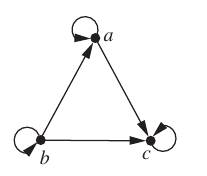
\includegraphics[scale=0.5]{img/9_3_24_digraph.png} \\
          \answer \\
          $\{(a,a),\ (a,c),\ (b,b),\ (b,a),\ (b,c),\ (c,c)\}$
\end{itemize}

\subsection{9.5}
\begin{itemize}
    \item[2.]  Which of these relations on the set of all people are equivalence relations? Determine the properties of an equivalence relation that the others lack.
          \begin{enumerate}[a.]
              \item $\{(a, b) \mid a \text{ and } b$ are the same age\}
              \item $\{(a, b) \mid a \text{ and } b$ have the same parents\}
              \item $\{(a, b) \mid a \text{ and } b$ share a common parent\}
              \item $\{(a, b) \mid a \text{ and } b$ have met\}
              \item $\{(a, b) \mid a \text{ and } b$ speak a common language\}
          \end{enumerate}
          \answer
          \begin{enumerate}[a.]
              \item equivalence relation
              \item equivalence relation
              \item missing transitive
              \item missing transitive
              \item missing transitive  
          \end{enumerate}

\end{itemize}
